\documentclass[12pt,a4paper]{article}

\usepackage[T1]{fontenc}
\usepackage[utf8]{inputenc}
\usepackage[brazil]{babel}
\usepackage{graphicx}
\usepackage{float}
\usepackage{geometry}

\geometry{margin=2.5cm}

\title{Introdu\c{c}\~ao ao LaTeX e sua Aplica\c{c}\~ao em Documentos Acad\^emicos}
\author{Samuel Henrique Carneiro Pereira}
\date{17 de abril de 2026}

\begin{document}

\maketitle

\section{Introdu\c{c}\~ao}
O LaTeX \'e um sistema de prepara\c{c}\~ao de documentos amplamente utilizado na produ\c{c}\~ao acad\^emica, especialmente em \'areas que exigem alta qualidade tipogr\'afica e organiza\c{c}\~ao consistente do conte\'udo. Sua principal vantagem est\'a na separa\c{c}\~ao entre conte\'udo e formata\c{c}\~ao, o que facilita a escrita de textos t\'ecnicos, relat\'orios e artigos cient\'ificos.

Neste mini-artigo, s\~ao apresentados alguns elementos b\'asicos do LaTeX, como se\c{c}\~oes, listas, inser\c{c}\~ao de imagens, tabelas e refer\^encias bibliogr\'aficas. Segundo \cite{silva2025}, o dom\'inio dessas estruturas contribui para uma produ\c{c}\~ao textual mais padronizada e profissional.

\section{Desenvolvimento}
Uma das caracter\'isticas mais importantes do LaTeX \'e a possibilidade de estruturar o documento de forma clara e objetiva. Em vez de editar visualmente cada detalhe, o autor define comandos que organizam o texto e mant\^em a uniformidade ao longo do arquivo.

Entre os recursos iniciais mais utilizados, destacam-se:

\begin{itemize}
    \item cria\c{c}\~ao autom\'atica de t\'itulos, autores e datas;
    \item divis\~ao do conte\'udo em se\c{c}\~oes bem definidas;
    \item inser\c{c}\~ao de figuras para complementar a explica\c{c}\~ao;
    \item uso de tabelas para apresentar dados de forma organizada.
\end{itemize}

A Figura \ref{fig:exemplo} ilustra a inser\c{c}\~ao de uma imagem no documento. Esse recurso \'e \'util para complementar o texto com representa\c{c}\~oes visuais.

\begin{figure}[H]
    \centering
    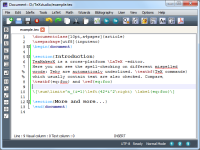
\includegraphics[width=0.75\textwidth]{texstudioimage.png}
    \caption{Interface do TeXstudio utilizada na edi\c{c}\~ao do documento.}
    \label{fig:exemplo}
\end{figure}

Tamb\'em \'e poss\'ivel apresentar informa\c{c}\~oes sint\'eticas em forma de tabela, como no exemplo abaixo.

\begin{table}[H]
    \centering
    \caption{Compara\c{c}\~ao simples entre editores de texto e LaTeX.}
    \begin{tabular}{|l|c|c|}
        \hline
        Recurso & Editor comum & LaTeX \\
        \hline
        Formata\c{c}\~ao autom\'atica & Parcial & Sim \\
        \hline
        Controle de refer\^encias & Limitado & Sim \\
        \hline
        Qualidade tipogr\'afica & M\'edia & Alta \\
        \hline
    \end{tabular}
\end{table}

Esses exemplos mostram que o LaTeX oferece uma base robusta para a escrita acad\^emica, mesmo em documentos simples e introdut\'orios.

\section{Conclus\~ao}
O uso do LaTeX permite produzir documentos organizados, leg\'iveis e adequados ao contexto acad\^emico. Mesmo com comandos b\'asicos, j\'a \'e poss\'ivel criar artigos com elementos essenciais, como lista, imagem, tabela e refer\^encia bibliogr\'afica.

Portanto, aprender os fundamentos do LaTeX \'e um passo importante para estudantes e profissionais que desejam melhorar a apresenta\c{c}\~ao de seus trabalhos escritos e adotar um padr\~ao mais t\'ecnico na elabora\c{c}\~ao de documentos.

\begin{thebibliography}{9}
\bibitem{silva2025}
SILVA, Mariana.
\textit{Escrita acad\^emica com LaTeX: fundamentos para iniciantes}.
S\~ao Paulo: Editora Exemplo, 2025.
\end{thebibliography}

\end{document}
